\documentclass{siproblemset}

% SI Session Information
\course{MTH 1321}       % the course of your SI
\sessionnum{17}         % (optional) specify the session number
\sessiondate{11/4/19}   % the date of the session

\warmup{Concept Review}
\topic{Curve Sketching}
\topic{Properties of Derivatives}
\cooldown{Graphing $f$ from $f'$/$f''$}

% Worksheet Information
\title{Analyzing and Sketching\linebreak Graphs of Functions}
\sections{Section 4.6}
\withnamespace

\begin{document}
    \maketitle
    
    \activity{Warmup}{Concept Review}{Work \textbf{alone} to answer this question. Try not to use your notes.}{15 minutes}
    
    \mcq[2]{The following graph is the graph of $f'$, the derivative of the twice-differentiable function $f$. Determine the following:}{
        \task The $x$-values of local extrema
        \task The $x$-values of inflection points
        \task Intervals of increase and decrease of $f$
        \task Intervals where $f$ is concave up and down
    }
    
    \begin{center}
        \mbox{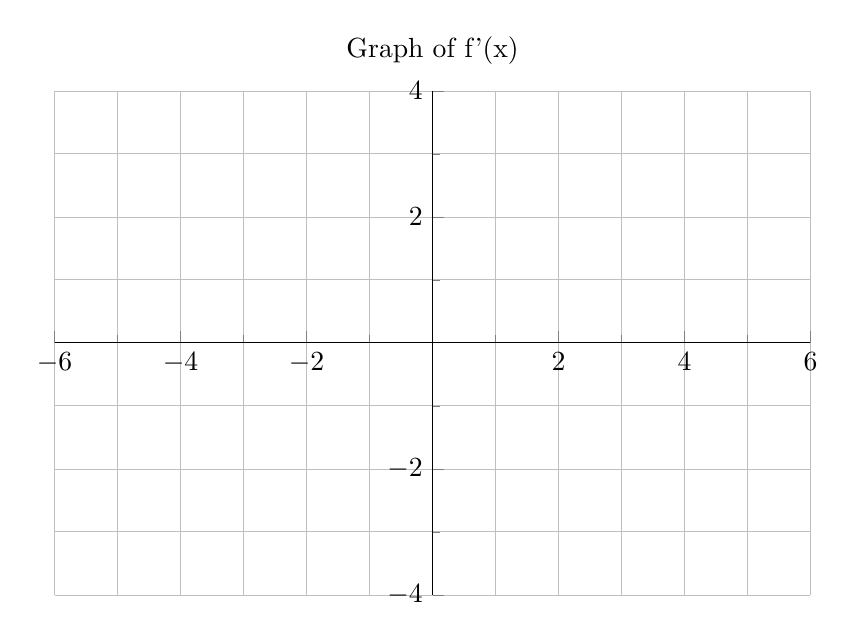
\begin{tikzpicture}[baseline=(current bounding box.north)]
            \begin{axis}[
            title={Graph of f'(x)},
            x=0.8cm,
            y=0.8cm,
            xmin=-6,
            xmax=6,
            ymin=-4,
            ymax=4,
            grid=both,
            major grid style={line width=.2pt,draw=gray!50},
            minor tick num=1,
            axis x line*=middle,
            axis y line*=middle,
            every axis plot/.append style={ultra thick},
            samples=200
            ]
            \end{axis}
            \end{tikzpicture}}
    \end{center}
    \newpage
    
    \activity{Activity 1}{Curve Sketching}{Make a \textbf{group of two or three, all with the same colored worksheets,} to work together to answer your assigned question. Then, try to answer the other question. Try not to use your notes. \textbf{DO NOT use a calculator}.}{30 minutes}
    
    \frq{Sketch the curve of $y=\dfrac{1}{x}+\dfrac{1}{x-1}$.}
    \newpage
    \frq{Sketch the curve of $y=\dfrac{x^3-1}{x}$.}
    \newpage

    \activity{Activity 2}{Properties of Derivatives}{Make a \textbf{group of two or three, all with different colored worksheets,} to answer your assigned question. Then, try to answer the other questions. Try not to use your notes. \textbf{DO NOT use a calculator}.}{30 minutes}
    
    \frq{Show that $f(x)=x^3-3x^2+6x$ has a point of inflection but no local extreme values.}
    \Hugesp
    \mcq[4]{Draw the graph of a function $f$ having the given limits at $\pm\infty$ and for which $f'$ and $f''$ take on the given sign combinations (pairs) in order.}{
        \task $\lim\limits_{x\to-\infty}=-1$
        \task $\lim\limits_{x\to\infty}=1$
        \task* $\text{sign}(f',f''): ++\rightarrow+-\rightarrow--\rightarrow-+$
    }
\newpage
    \frq{State the sign change at each transition point $A$--$G$ on the graph. Example: $f'(x)$ goes from $+$ to $-$ at $A$.}
\begin{center}
    \includegraphics[width=0.5\linewidth]{../../../../Desktop/graph}
\end{center}
\end{document}